\documentclass[10pt]{beamer} %with transitions 
%\documentclass[handout, 10pt]{beamer}  %without transitions

%\documentclass[notes]{beamer}       % print frame + notes
%\documentclass[notes=only]{beamer}   % only notes
%\documentclass{beamer}              % only frames
%\usepackage[utf8]{inputenc}


\setbeamertemplate{note page}[plain]
%\setbeameroption{show notes} 

\setbeamertemplate{footline}[frame number]

\usepackage[style = phys]{biblatex}
\addbibresource{biblio.bib}
\usepackage{url}
\usepackage{subfigure} 
 

\makeatletter
\long\def\beamer@@ssection*#1{\beamer@section[]{}}
\makeatother

\usepackage{physics}

\usepackage{amsmath}
\usepackage{tikz}
\usetikzlibrary{tikzmark}
\setbeamertemplate{caption}[numbered]

\newcommand{\nl}{\\ \vspace{1em}}

\mode<presentation> {

% The Beamer class comes with a number of default slide themes
% which change the colors and layouts of slides. Below this is a list
% of all the themes, uncomment each in turn to see what they look like.

%\usetheme{default}
%\usetheme{AnnArbor}
%\usetheme{Antibes}
%\usetheme{Bergen}
%\usetheme{Berkeley}
%\usetheme{Berlin}
%\usetheme{Boadilla}
%\usetheme{CambridgeUS}
%\usetheme{Copenhagen}
%\usetheme{Darmstadt}
%\usetheme{Dresden}
%\usetheme{Frankfurt}
%\usetheme{Goettingen}
%\usetheme{Hannover}
\usetheme{Ilmenau}
%\usetheme{JuanLesPins}
%\usetheme{Luebeck}
%\usetheme{Madrid}
%\usetheme{Malmoe}
%\usetheme{Marburg}
%\usetheme{Montpellier}
%\usetheme{PaloAlto}
%\usetheme{Pittsburgh}
%\usetheme{Rochester}
%\usetheme{Singapore}
%\usetheme{Szeged}
%\usetheme{Warsaw}

% As well as themes, the Beamer class has a number of color themes
% for any slide theme. Uncomment each of these in turn to see how it
% changes the colors of your current slide theme.

%\usecolortheme{albatross}
%\usecolortheme{beaver}
%\usecolortheme{beetle}
%\usecolortheme{crane}
%\usecolortheme{dolphin}
%\usecolortheme{dove}
%\usecolortheme{fly}
%\usecolortheme{lily}
%\usecolortheme{orchid}
%\usecolortheme{rose}
%\usecolortheme{seagull}
%\usecolortheme{seahorse}
%\usecolortheme{whale}
%\usecolortheme{wolverine}

%\setbeamertemplate{footline} % To remove the footer line in all slides uncomment this line
%\setbeamertemplate{footline}[page number] % To replace the footer line in all slides with a simple slide count uncomment this line

%\setbeamertemplate{navigation symbols}{} % To remove the navigation symbols from the bottom of all slides uncomment this line
}

\usepackage{multicol} %used for multiple columns

\usepackage{graphicx} % Allows including images
\usepackage{booktabs} % Allows the use of \toprule, \midrule and \bottomrule in tables

\usepackage{braket} %quantum brackets



%----------------------------------------------------------------------------------------
%	TITLE PAGE
%----------------------------------------------------------------------------------------

\title[Search for a heavy Higgs boson decay $A \to ZH \to  \ell\ell bb$ final state in $pp$ collisions at $\sqrt{s} = 13$ TeV with the ATLAS detector]{Search for a heavy Higgs boson decaying into a Z boson and another heavy Higgs boson in the $\ell\ell bb$ final state in $pp$ collisions at $\sqrt{s} = 13$ TeV with the ATLAS detector} % The short title appears at the bottom of every slide, the full title is only on the title page
\author[Daniel Prelipcean]{Daniel Prelipcean} % Your name
\institute[Physics at LHC - Advanced Seminar] % Your institution as it will appear on the bottom of every slide, may be shorthand to save space
{Technical University of Munich\\Physics at LHC - Advanced Seminar}
\date{December 16$^{th}$, 2019} % Date, can be changed to a custom date



\begin{document}

\begin{frame}
\titlepage % Print the title page as the first slide

\end{frame}



%----------------------------------------------------------------------------------------
%	PRESENTATION SLIDES
%----------------------------------------------------------------------------------------

%------------------------------------------------
%===================================================



\section{2HDM}

\begin{frame}
\frametitle{Reasons for BSM Physics}
Unanswered questions:
\begin{enumerate}
    \item Supersymmetry
    \item Dark matter
    \item Axions and the Strong CP Problem
    \item Electroweak baryogenesis
    \item Neutrino masses and mixings
    \item Hierarchy problem
\end{enumerate}
indicate that physics beyond SM must exist. \\

The Two-Higgs-doublet model (2HDM) is one of the simplest extensions of the SM.

\end{frame}

\note{2HDM models are one of the natural choices for beyond SM models containing two Higgs doublets instead of just one. There are also models with more than two Higgs doublets example three Higgs doublet models etc.}


\begin{frame}{Higgs Field (SM)}
The Higgs field is a four-component scalar field, with two neutral and two electrically charged components that form a complex doublet of the weak isospin $SU(2)$ symmetry. 

\begin{equation}
\phi ={\frac {1}{\sqrt {2}}}\left({\begin{array}{c}\phi ^{1}+i\phi ^{2}\\\phi ^{0}+i\phi ^{3}\end{array}}\right)
\end{equation}



SM uses only 2 parameters:
\begin{itemize}
    \item $m_h \approx (125.18 \pm 0.16)\,{\rm {GeV}}/c^2$, the higgson mass
    \item $v\approx 246.22\,{\rm {GeV}}$, its vacuum expectation value 
\end{itemize}

and the potential is:
\begin{equation}
    V = − \mu^2 \phi^\dagger + \frac{1}{2} \lambda (\phi^\dagger \phi )^2 
\end{equation}

\end{frame}

\begin{frame}{Two Higgs Double Model (2HDM)}
It contains two Higgs doublets instead of just one, with five physical scalar states:
\begin{itemize}
    \item the CP even neutral Higgs bosons $h$ and $H$ (with $m_H > m_h$)
    \item  the CP odd pseudoscalar $A$
    \item  two charged Higgs bosons $H^{\pm }$
\end{itemize}
The discovered higgson is strongly hinted to be CP even so it is likely they can be mapped either $h$ or $H$. \\

This leads to a richer phenomenology.\\

\end{frame}



\begin{frame}{2HDM Parameter Space}
The 2HDM potential can be generically writen as:
    \begin{equation*}
        V = m_{11}^2 \phi_1^\dagger \phi_1 + m_{22}^2 \phi_2^\dagger \phi_2 - (m_{12}^2 \phi^\dagger_1 \phi_2 + H.C.) + V_{model}
    \end{equation*}
    where $V_{model}$ depends on the specific 2HDM type and the $m_{12}$ factor is called the 2HDM parameter.\\
Such a model can be described via six physical parameters: 
\begin{itemize}
    \item $m_{h},m_{H},m_{A},m_{{H^{\pm }}}$: four Higgs masses
    \item $\tan \beta = \dfrac{v_1}{v_2}$: the ratio of the two doublets vacuum expectation values; it also represents rotation angle which diagonalizes the mass-squared matrices of the charged scalars and of the pseudoscalars
    \item $\alpha $: the mixing angle which diagonalizes the mass matrix of the neutral CP even Higgses.
\end{itemize}
\end{frame}



\begin{frame}{Special cases}
The two parameters $\alpha$ and $\beta$ determine the interactions of the various Higgs fields with the
vector bosons and (given the fermion masses) with the fermions:
\begin{enumerate}
    \item $ \cos(\beta -\alpha )\rightarrow 0$, the \emph{alignment limit}:
     \begin{itemize}
         \item the lighter CP even Higgs boson $h$ has couplings exactly like the SM-Higgs boson
         \item the heavier $H$ couples to just fermions ("gauge-phobic")
     \end{itemize}
    \item $ \sin(\beta -\alpha )\rightarrow 0$:
    \begin{itemize}
        \item the heavier CP even boson, and $H$ is SM-like
        \item leaving $h$ to be the lighter than the discovered Higgs, and it couples just to gauge bosons ("fermio-phobic")
    \end{itemize}
\end{enumerate}
but not both.
        
\end{frame}


\begin{frame}{2HDM solutions for (some of) the unanswered questions}
    \begin{itemize}
        \item Supersimmetry requires at least two Higgs doublets:\\
        eg. the Minimal Supersymmetric Standard Model (MSSM)
        \item Axion models: possible CP-violating term in the QCD Lagrangian, can be rotated away if the Lagrangian contains a global U(1) symmetry. \\
        Imposing this symmetry requires two Higgs doublets.
        \item Baryon asymmetry:  2HDM has a scalar mass spectrum flexibility and additional sources of CP violation, either explicit or spontaneous
    \end{itemize}
    
\end{frame}


\section{Channels}

\begin{frame}{Guiding principles}
The key method to distinguish between these different models involves a study of:
\begin{itemize}
    \item particles' interactions ("coupling")
    \item exact decay processes ("branching ratios")
\end{itemize}
which can be measured and tested experimentally in particle collisions.\\
    
\end{frame}


\begin{frame}{LHC Searches}

There have been many searches for the
heavy neutral Higgs bosons of the 2HDM at the LHC:
\begin{enumerate}
    \item $H \to WW/Z Z$
    \item $A \to Z H$ 
    \item $H \to hh$
    \item $A/H \to \tau \tau /bb$
[14–16]
\end{enumerate}
\end{frame}

\begin{frame}{Production channels (1)}
\begin{itemize}
    \item For large parts of the 2HDM parameter space, the dominant CP-odd Higgs boson decay channel is $A \to ZH$. 
    \item This search for $A \to ZH$ decays uses proton–proton collision data at $\sqrt{s} = 13$ TeV corresponding to an integrated luminosity of $36.1$ fb$^{−1}$ recorded by the ATLAS detector at the LHC. 
   
\end{itemize}
\end{frame}

\begin{frame}{Production channels (2)}
     The production of the A boson in the relevant 2HDM parameter space proceeds mainly through:

    \begin{figure}
        \centering
        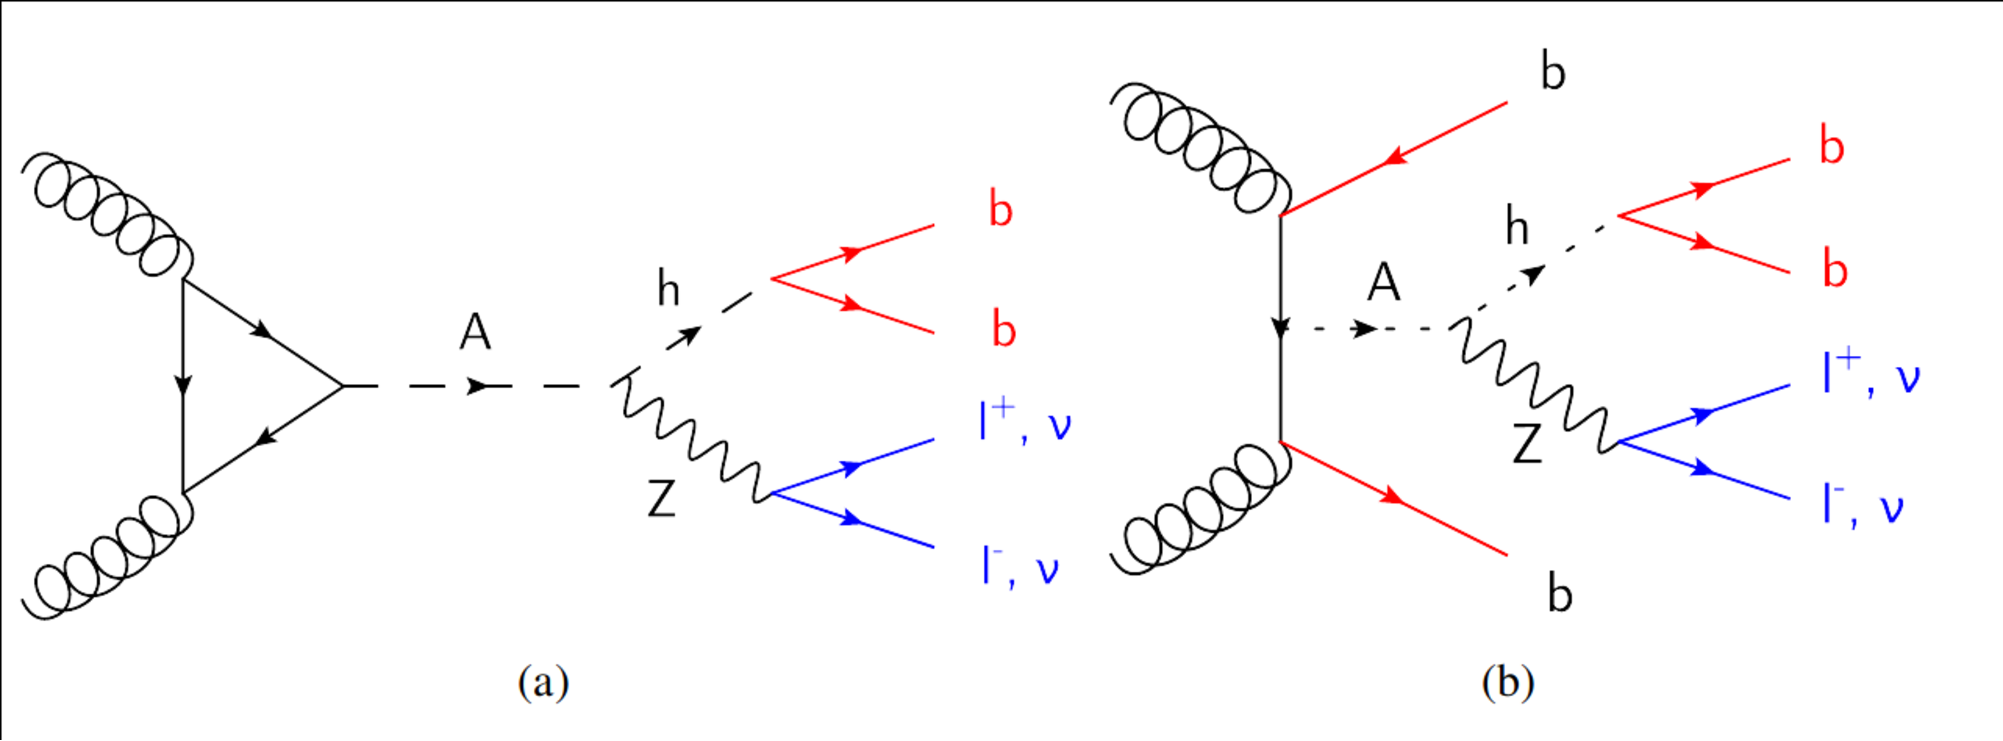
\includegraphics[width=1.0\textwidth]{Figs/FeynmanGraph_PseudoScalarProduction.pdf}
    \end{figure}    


\end{frame}


\begin{frame}{Channel selection}
The search considers only:
\begin{itemize}
    \item $Z \to \ell\ell$, where $\ell = e, \mu$, for the clean leptonic final state $\ell \ell b b$
    \item $H \to bb$, because of its large branching ratio.
\end{itemize}

This final state:
\begin{itemize}
    \item is fully constrained: allows full reconstruction of the A boson decay kinematics.
    \item has less background noise
    \item has smallest Higgs signal
\end{itemize} 

\end{frame}


\begin{frame}{Jets and flavour tagging}

\begin{block}{Jets}
    A jet is a narrow cone of hadrons and other particles produced by the hadronization of a quark or gluon
\end{block}

\begin{itemize}
    \item Particles carrying a color charge (quarks) cannot exist in free form because of QCD confinement.
    \item When an object containing color charge fragments, each fragment carries away some of the color charge. 
    \item In order to obey confinement, these fragments create other colored objects around them to form colorless objects. 
    \item The ensemble of these objects is called a jet, since the fragments all tend to travel in the same direction, forming a narrow "jet" of particles.
\end{itemize}

\end{frame}

\begin{frame}{b-tagging}
    \begin{block}{Tagging}
        \item  It is the identification (or "tagging") of jets originating from the same quark flavor, e.g. bottom quarks (or b quarks, hence the name).
\end{block}

Importance of b-tagging:
\begin{itemize}
    \item The physics of bottom quarks is quite interesting; in particular, it sheds light on CP violation.
    \item Some important high-mass particles (both recently discovered and hypothetical) decay into bottom quarks:
    \begin{itemize}
        \item Top quarks very nearly always do so 
        \item the Higgs boson is expected to decay into bottom quarks more than any other particle
    \end{itemize}
    \item  Identifying bottom quarks helps to identify the decays of these particles.
\end{itemize}


\end{frame}


\section{ATLAS Detector}

\begin{frame}{ATLAS Coordinat System}



\begin{figure}[ht]
        \centering
        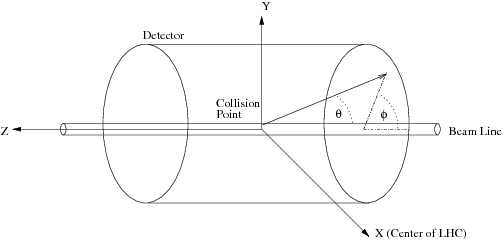
\includegraphics[width=1.0\textwidth]{Figs/atlas_coordinate_system.png}
        \caption{Atlas coordinate system}
        \label{fig:atlas-coordinate} 
\end{figure}

\end{frame}



\begin{frame}{ATLAS detector}
    
    \begin{figure}[ht]
        \begin{minipage}[b]{0.64\linewidth}
             \centering
            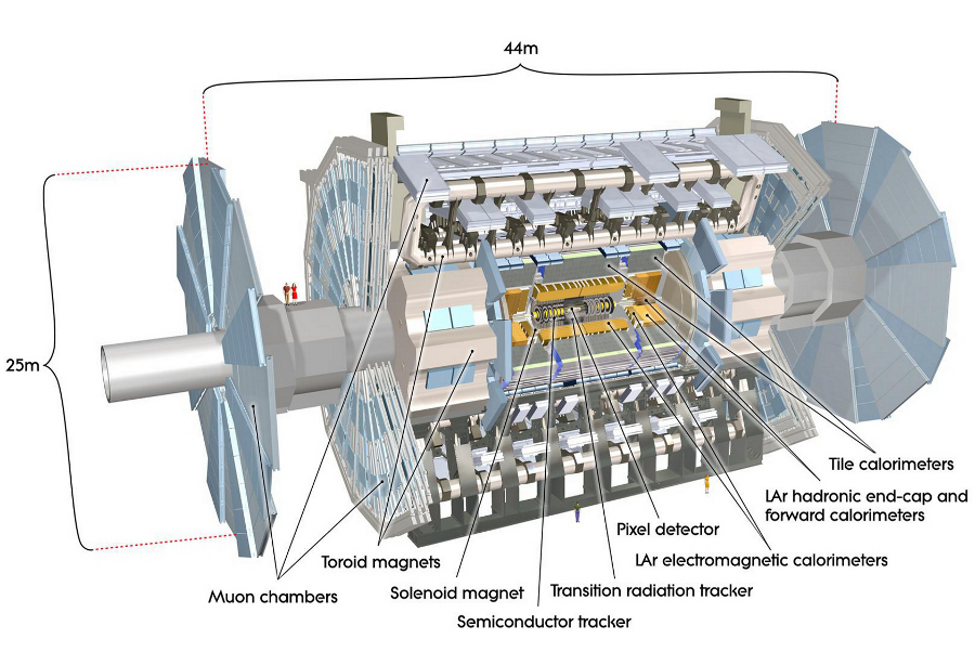
\includegraphics[width=1.00\textwidth]{Figs/atlas-detector.png}
%            \caption{Space-time probabilities}
%            \label{fig:a}
        \end{minipage}
        \hfill
        \begin{minipage}[b]{0.34\linewidth}
            \centering
            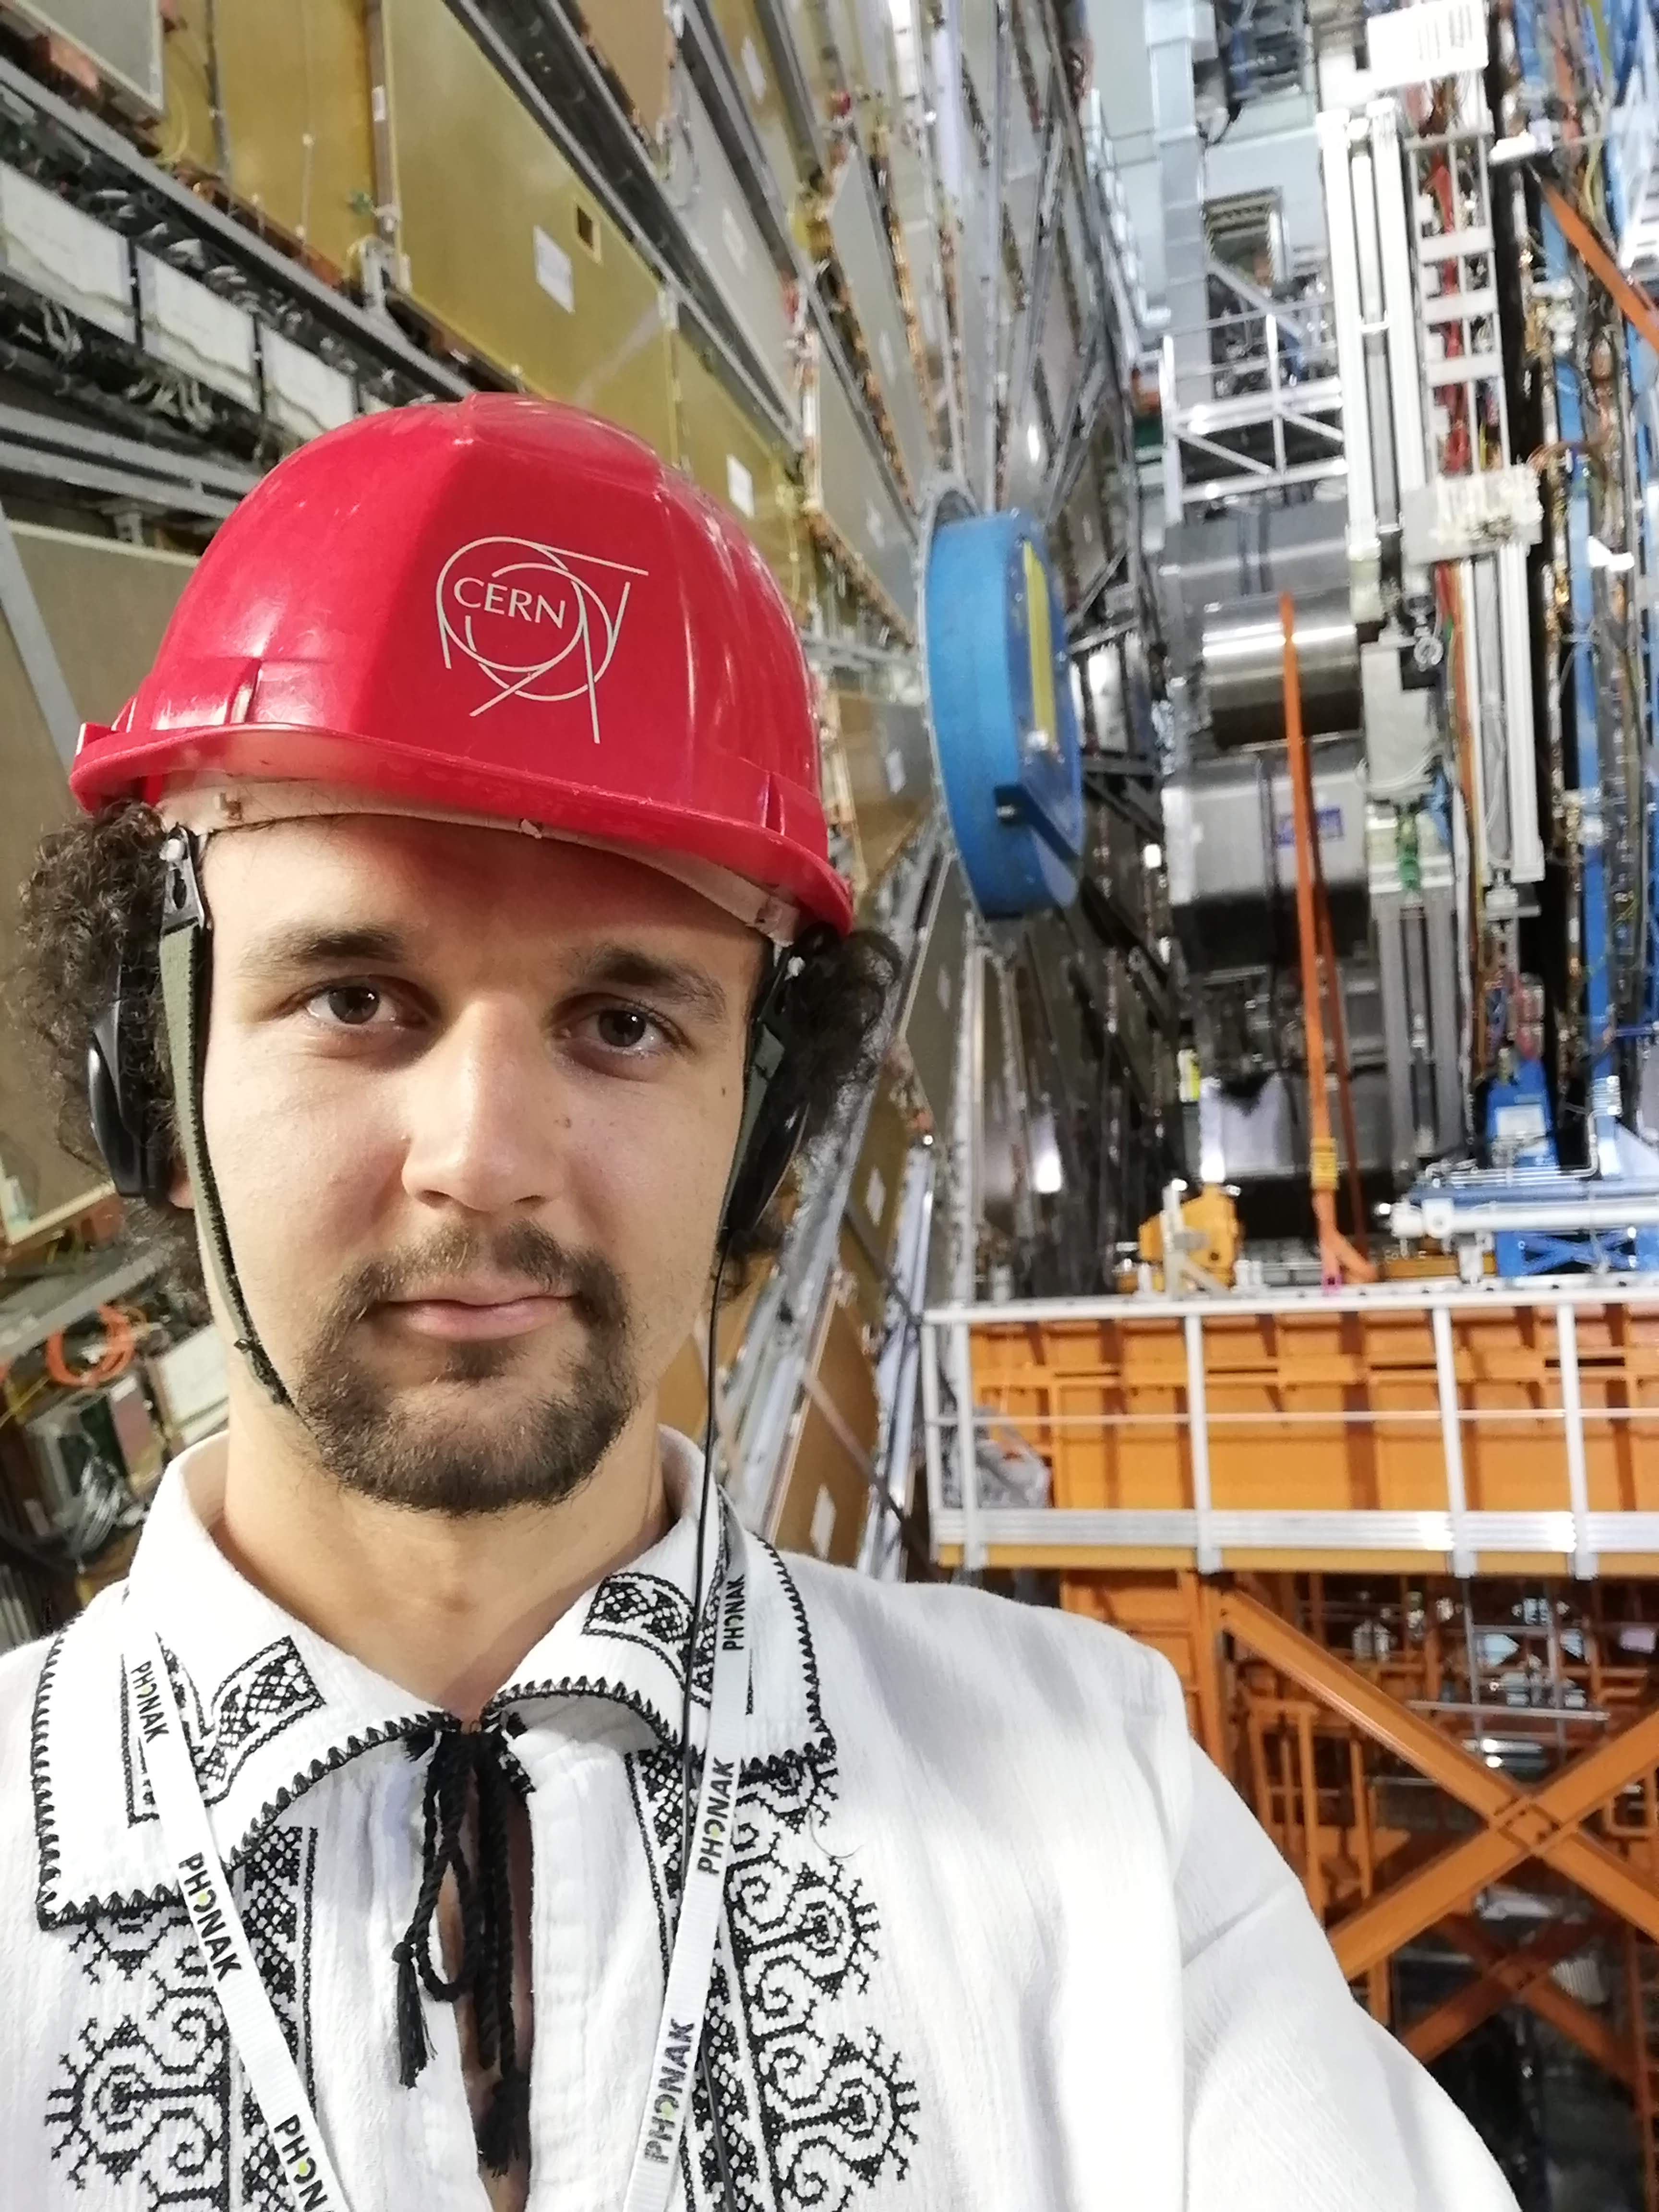
\includegraphics[width=1.00\textwidth]{Figs/atlas-my-pic.jpg}
 %           \caption{Gaussian Spreading \cite{Pavsic}}
 %           \label{fig:b}
        \end{minipage}
\end{figure}

\end{frame}





\begin{frame}{Definitions}
\begin{block}{Pseudorapidity}
In terms of the polar angle $\theta$, as $\eta = - \ln {\tan(\theta/2)}$
\end{block}    

\begin{block}{Transverse momenta $p_T$}
Computed from the three-momenta $\vec{p}$ as $p_T= |\vec{p}| \sin{\theta}$
\end{block}    

\end{frame}
%===================================================



\begin{frame}{Reconstructed particles}
    

\begin{block}{Electrons}
    \begin{itemize}
        \item Detected in the electromagnetic calorimeter
        \item Effciency to be reconsructed and meet criteria: 85\% for $p_T > 7$ GeV and 90\% for $p_T > 27$ GeV
    \end{itemize}
\end{block}

\begin{block}{Muons}
    \begin{itemize}
        \item Detected in muon spectrometer
        \item Efficiency 97\% for $|\eta|<2.5$ and $p_T >7$ GeV
    \end{itemize}
\end{block}

\begin{block}{Jets}
\begin{itemize}
    \item Detected in calorimeter system
    \item Candidates are required to have: $p_T >20$ GeV at $|\eta|<2.5$ and $p_T >30$ GeV at $2.5<|\eta|<4.5$ 
\end{itemize}

\end{block}

\end{frame}



\section{Analysis Strategy}

\begin{frame}{Resonance of interest}

    \begin{block}{Resonance}
     The peak located around a certain energy found in differential cross sections of scattering experiments. In common usage, "resonance" only describes particles with very short lifetimes, mostly high-energy hadrons existing for $10^{-23}$ seconds or less.
    \end{block}

\begin{block}{The pseudoscalar boson resonance}
\begin{equation*}
        A \to ZH \to \ell\ell b b
\end{equation*}

\end{block}

    \begin{minipage}[b]{0.32\linewidth}
        \centering
\uncover<2->{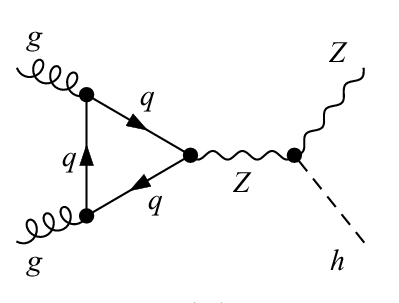
\includegraphics[width=1.0\textwidth]{Figs/ZHbkg1.png}}
    \end{minipage}
        \hfill
    \begin{minipage}[b]{0.32\linewidth}
        \centering
        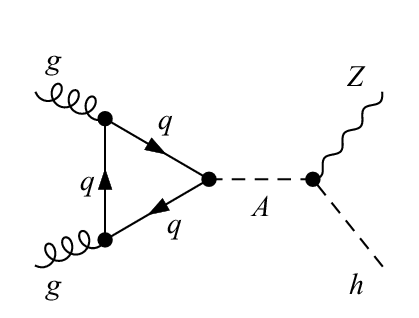
\includegraphics[width=1.0\textwidth]{Figs/AtoZH.png}
    \end{minipage}
        \hfill
    \begin{minipage}[b]{0.32\linewidth}
        \centering
\uncover<2->{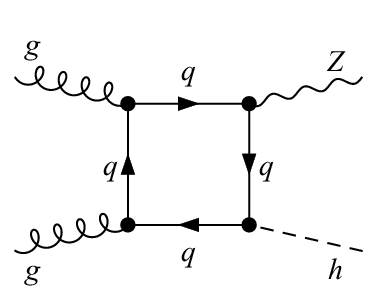
\includegraphics[width=1.0\textwidth]{Figs/ZHbkg2.png}}
    \end{minipage}


    
\end{frame}


\begin{frame}{Most Relevant Background Resonances}
    
    \begin{minipage}[b]{0.49\linewidth}
        \centering
        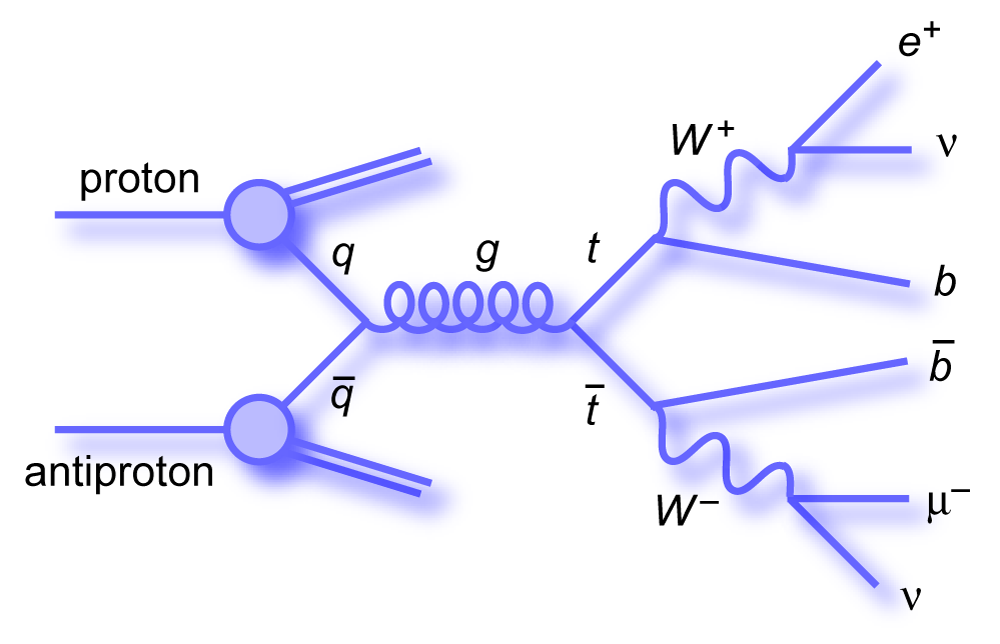
\includegraphics[width=1.0\textwidth]{Figs/feynman_ttbar_emu.png}
        \caption{$t\bar{t}$}
    \end{minipage}
        \hfill
    \begin{minipage}[b]{0.49\linewidth}
        \centering
        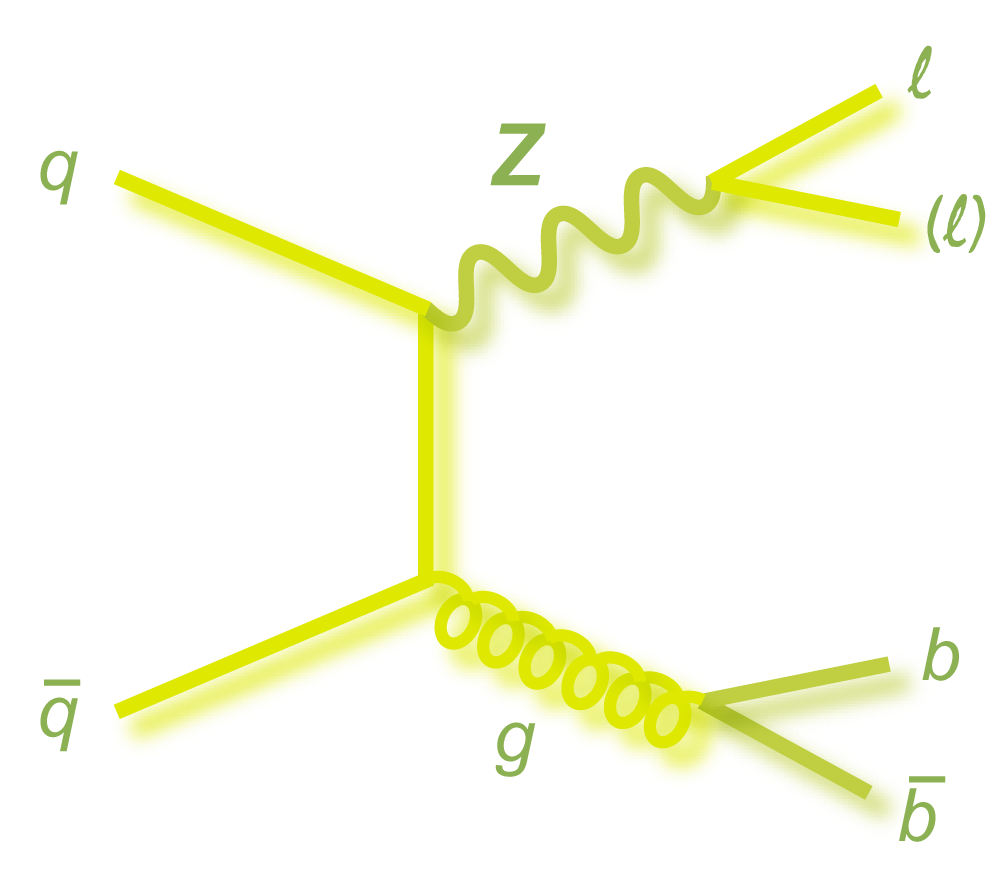
\includegraphics[width=1.0\textwidth]{Figs/feynman_Z_llbb.png}
        \caption{$Z+$jets}
    \end{minipage}

\end{frame}


\begin{frame}{Control regions}

\begin{itemize}
    \item The $t\bar{t}$ and $Z+$ jets control regions are included in the likelihood calculation, to help constrain their respective contribution in the signal region
    \item Achieved via two free normalisation scale factors $\vec{\alpha}$.
    \item Values estimated from the simulation and determined from the fit. Typical values are close to unity, e.g.:\\
    for $(m_A, M_H)=(700, 200)$ GeV:
    \begin{itemize}
        \item $\alpha_{Z+jets}=1.12 \pm 0.09$
        \item $\alpha_{t\bar{t}}=0.96\pm0.06$
    \end{itemize}
\end{itemize}

\end{frame}

\begin{frame}{Missing transverse energy}

    \begin{block}{Primary vertex}
        Taken to be the reconstructed vertex with the highest $\Eta p_T^2$ of the associated tracks.
    \end{block}

    \begin{block}{Missing Transverse Energy $E_T^{miss}$}
        Computed using \emph{reconstructed} and \emph{calibrated} leptons, photons and jets tracks from primary vertex.\\
        It is used to infer the presence of non-detectable particles (e.g. neutrinos)
    \end{block}

\end{frame}


\begin{frame}{Possible resonances}
    Several resonances leading to an $\ell\ell bb$ final state, hence several cuts to focus on the $A$ decay:
    \begin{itemize}
        \item $H \to bb$ reconstructed by requiring at least two b-jets with highest $p_T$ one having $p_T>45$ GeV. \\
        Reduce by requiring $E_T^{miss}/ \sqrt{p_T}<3.5$ GeV
        \item reduce the Z+jets background: $\sqrt{\Eta p_T^2}/m_{\ell\ell bb} > 0.4$, where $m_{\ell\ell bb}$ is the four body invariant mass
        \item the invariant mass of the two leading b-jets must be compatible with the assumed H boson mass:
            \begin{equation}
                0.85 \cdot m_H - 20 GeV < m_{bb} < m_H + 20 GeV
            \end{equation}
    \end{itemize}
\end{frame}

\begin{frame}{Analysis Strategy}
The $m_{\ell\ell bb}$ distribution after the $m_{bb}$ requirement is used to discriminate between signal and background.
    \begin{itemize}
        \item     To improve resolution:
         \begin{itemize}
             \item the $\ell\ell$ system's four momentum are scaled to match the $Z$ boson mass 
             \item the $bb$ system's four momentum components are scaled to match the assumed $H$ boson mass
         \end{itemize}
        \item     This procedure improves the $m_{\ell\ell bb}$ resolution by a factor of 2 without significantly distorting the background distribution.
    \end{itemize}

\end{frame}

\section{Fit models}

\begin{frame}{Fit models}
    \begin{itemize}
        \item     The following fits are done in order to interpolate between various discrete mass points that are put through the full detector and reconstruction chain.
        \item Distributions of interest: Gaussian, EGE, DCSB, Breit-Wigner

    \end{itemize}



\end{frame}

\begin{frame}{Distributions}
\begin{itemize}
    \item If the decay with is negligible compared to the detector resolution: EGE and DCSB.

    \item Both functions consist of a Gaussian core with mean $a$ and variance $\sigma$, while the rest of the parameters describe the tails.

    \item The small differences in the tails of some distributions between the functional forms and the simulations:
    \begin{itemize}
        \item have only negligible effects on the final results
        \item are included as source of systematic uncertainty.    
    \end{itemize}
    
\end{itemize}
\end{frame}

\begin{frame}{Distributions: EGE}
    \begin{itemize}
        \item[i)] ExpGaussExp (EGE):
        \begin{equation}
            f_{EGE}(m; a, \sigma, k_L, k_H) = \begin{cases}
\exp{\dfrac{1}{2}k_L^2 + k_L\dfrac{m-a}{\sigma}}, for \dfrac{m-a}{\sigma} \leq - k_L \\
\exp{-\dfrac{1}{2}\left( \dfrac{m-a}{\sigma} \right)^2}, for - k_L < \dfrac{m-a}{\sigma} \leq k_H\\
\exp{\dfrac{1}{2}k_H^2 - k_H\dfrac{m-a}{\sigma}}, for \dfrac{m-a}{\sigma} >  k_H \\
\end{cases}
        \end{equation}
    \end{itemize}
        

\end{frame}

\begin{frame}{Distributions: DCSB}

\begin{itemize}
    \begin{itemize}
        \item[ii)] double Gaussian Crystal Ball (DCSB):
\begin{align*}
    f_{DCSB} & (m; a, \sigma, k_L, k_H, n_1, n_2) = \\ 
    & = \begin{cases}
g(m;a, -\sigma, k_L, n_1)\cdot \exp{-\dfrac{1}{2}k_L^2}, for \dfrac{m-a}{\sigma} \leq - k_L \\
\exp{-\dfrac{1}{2}\left( \dfrac{m-a}{\sigma} \right)^2}, for - k_L < \dfrac{m-a}{\sigma} \leq k_H\\
g(m; a, \sigma, k_H,n_2)\cdot\exp{\dfrac{1}{2}k_H^2}, for \dfrac{m-a}{\sigma} >  k_H
\end{cases}
\end{align*}
where $g(m;a, \sigma,k,n) = \left[ \frac{|k|}{n} \left(\frac{n}{|k|} - |k| + \frac{m-a}{\sigma} \right) \right]^{-n}$
    \end{itemize}
\end{itemize}


\end{frame}




\begin{frame}{Breit-Wigner distribution}
    \begin{itemize}
        \item     Used for the case when the $A$ boson's width is significant compared with the detector resolution while the $H$ boson's width remains negligible.
        \item     The relativistic Breit–Wigner distribution (after the 1936 nuclear resonance formula of Gregory Breit and Eugene Wigner) is a continuous probability distribution with the following probability density function:
        \begin{equation}
        f(E) = \frac{k}{\left(E^2-M^2\right)^2+M^2\Gamma^2}
        \end{equation}
        where the constant of proportionality is $k = \frac{2 \sqrt{2} M \Gamma  \gamma }{\pi \sqrt{M^2+\gamma}}$ with $\gamma=\sqrt{M^2\left(M^2+\Gamma^2\right)}$ 

    \end{itemize}
\end{frame}


\begin{frame}{Breit-Wigner distribution (2)}
    \begin{minipage}[b]{0.49\linewidth}
        \centering
        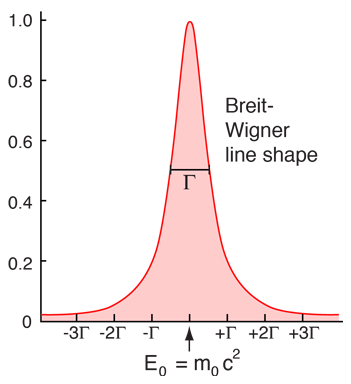
\includegraphics[width=1.0\textwidth]{Figs/BreitWigner.png}
    \end{minipage}
        \hfill
    \begin{minipage}[b]{0.49\linewidth}
        \begin{equation}
        f(E) = \frac{k}{\left(E^2-M^2\right)^2+M^2\Gamma^2}
        \end{equation}
        It is most often used to model resonances (unstable particles) in high-energy physics:
        \begin{itemize}
            \item $E$ is the center-of-mass energy that produces the resonance
            \item $M$ is the mass of the resonance
            \item $\Gamma$ is the resonance width (or decay width), related to its mean lifetime according to $\tau = 1/\Gamma$. 
        \end{itemize}
    \end{minipage}
\end{frame}


\begin{frame}{Fit Model}
    \begin{minipage}[b]{0.49\linewidth}
        \centering
        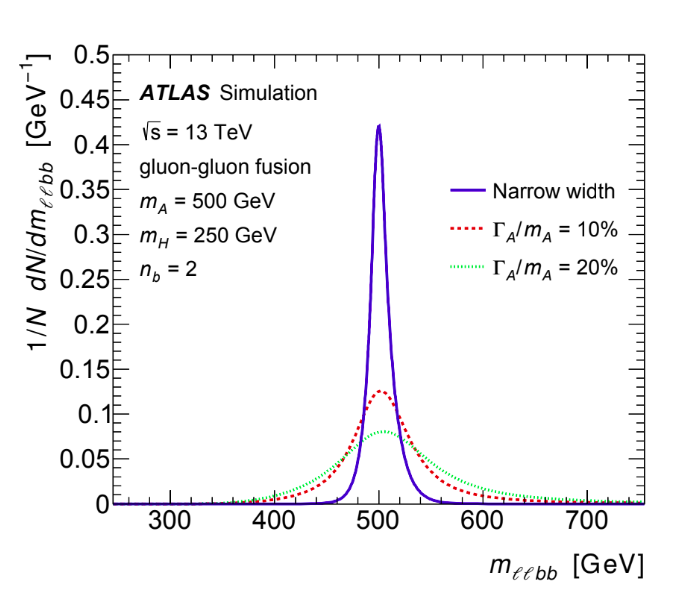
\includegraphics[width=1.0\textwidth]{Figs/model.png}
    \end{minipage}
        \hfill
    \begin{minipage}[b]{0.49\linewidth}
        \begin{itemize}
            \item         In order to model the $m_{\ell\ell bb}$ shape of A bosons with large natural widths, a modified Breit–Wigner distribution is convolved with the EGE and DSCB functions.
            \item The procedure is validated by comparing the results of the convolution with those of the simulated samples of A bosons with large natural widths. Widths of up to
20\% of the A boson mass are considered.
        \end{itemize}

    \end{minipage}

    
\end{frame}

\begin{frame}{Fit model}
    
    \begin{itemize}
        \item     The $m_{\ell\ell bb}$ distribution is expected to exhibit:
        \begin{itemize}
            \item a resonant structure if signal events are present
            \item a smooth shape from background events
        \end{itemize}

        \item The shape difference in the $m_{\ell\ell bb}$ distribution between the signal and the background contributions are exploited through binned maximum-likelihood fits of the signal-plus-background hypotheses.
    \end{itemize}

\end{frame}

\begin{frame}{Fit parameters}
    For a given mass hypothesis of $(m_A, m_H)$, the likelihood is constructed as the product of Poisson statistics in $m_{\ell\ell bb}$ bins:
    
    \begin{equation}
        L(\mu, \vec{\alpha}, \vec{\theta}| m_A, m_H) = \prod_{i=bins} Poisson \left( N_i | \left( \mu \times S_i (m_A, m_H, \vec{\theta}) + B_i(\vec{\alpha}, \vec{\theta}) \right) \right) \cdot G(\vec{\theta})
    \end{equation}
    
\begin{itemize}
    \item $N_i$ is the number of observed events
    \item $S_i (m_A, m_H, \vec{\theta}$ and $B_i(\vec{\alpha}, \vec{\theta})$ are signal and background in bin i
    \item $\vec{\alpha}$ is the free background normalisation scale factors
    \item $\mu$ multiplicative factor to the expected signal rate and is called the signal-strength parameter (from systematic uncertainties)
    \item $\vec{\theta}$ denotes all explicitly non-listed parameters of the likelihood function
\end{itemize}
    
\end{frame}

\section{Systematic Uncertainties}


\begin{frame}{Signal strength parameter $\mu$}
    \begin{itemize}
        \item     The effect of the systematic uncertainties on the search is studied using the signal-strength parameter $\mu$ for hypothesised signal production.
        \item Systematic Uncertainties are incorporated in the likelihood as nuisance parameters with either Gaussian or log-normal constraint terms.
    \end{itemize}

\end{frame}

\begin{frame}{Systematic Uncertainties}
    \begin{block}{A) Experimental Uncertainties}
    
        \begin{minipage}[b]{0.49\linewidth}
            \begin{itemize}
                \item luminosity measurement
                \item trigger
                \item object identification
            \end{itemize}

        \end{minipage}
        \hfill
        \begin{minipage}[b]{0.49\linewidth}
            \begin{itemize}
                \item energy/momentum scale
                \item resolution
                \item underlying event and pile-up
            \end{itemize}
        \end{minipage}

    \end{block}

    \begin{block}{B) Theoretical Uncertainties}
Modelling for:
    \begin{itemize}
        \item signal: 
        \begin{itemize}
            \item factorisation and renormalisation scale choice
            \item the initial- and final-state radiation treatment
            \item PDF choice
        \end{itemize}
        
        \item background: modelling of the $m_{bb}$ mass and the $p_{T}^{\ell\ell}$ distribution of Z+jets.
    \end{itemize}
    
    \end{block}

\end{frame}


\begin{frame}{Uncertainties Contributions}

    \begin{figure}
        \centering
        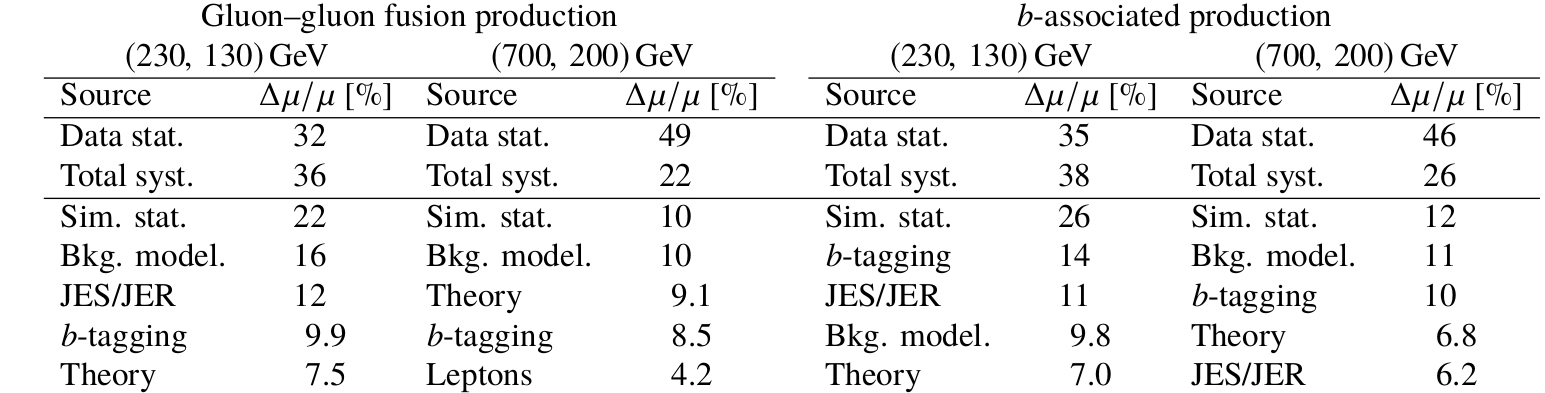
\includegraphics[width=0.95\textwidth]{Figs/uncertainties_table.jpg}
    \end{figure}
    
\end{frame}


\section{Results}

\begin{frame}{Results}

    \begin{block}{Step size}
    The scan is performed in steps of 10 GeV for:

    \begin{itemize}
        \item $m_A$ range 230-800 GeV
        \item $m_H$ range 130-700 Gev
    \end{itemize}
    such that $m_A - m_H \geq 100$ GeV
    \end{block}

    Step size chosen to be compatible with the detector resolution.
\end{frame}



\begin{frame}{$m_{\ell\ell b b}$ distribution: gluon-gluon fusion}
        \centering
        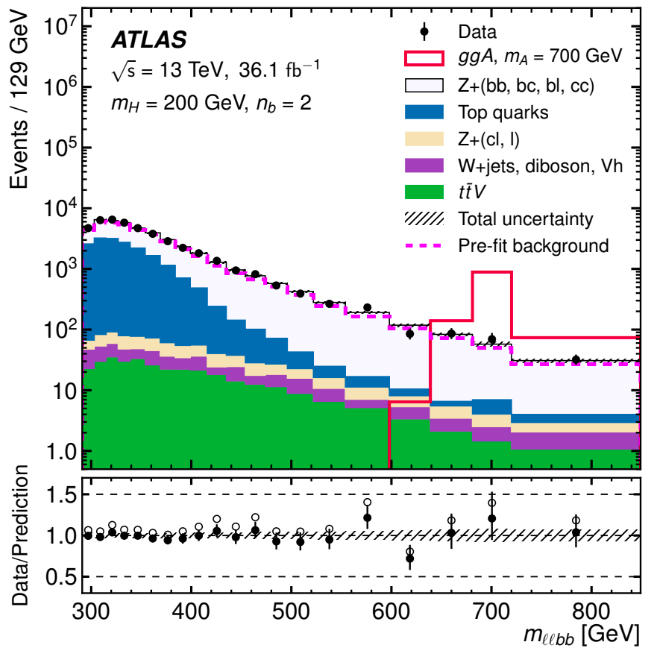
\includegraphics[width=0.6\textwidth]{Figs/mllbb_distribution.png}
        \caption{}
        \label{fig:mllbb-distribution} 
\end{frame}

\begin{frame}{$m_{\ell\ell b b}$ distribution: b jets associates}
        \centering
        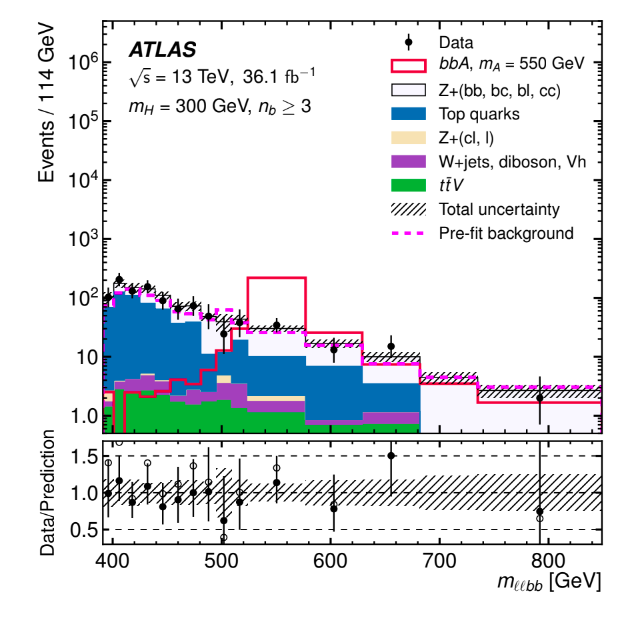
\includegraphics[width=0.6\textwidth]{Figs/mllbb_distribution_bb.png}
        \caption{}
        \label{fig:mllbb-distribution} 
\end{frame}


\begin{frame}{Background model comparison}
    Measured data is found to be well described by the background model. Some excesses are present at:
    \begin{itemize}
        \item gluon-gluon fusion production at $(m_A, m_H) = (750, 610)$ GeV with significance 3.5 (2.0)
        \item b-associated production at $(m_A, m_H) = (510, 310)$ GeV with significance 3.0 (1.2)
    \end{itemize}
\end{frame}

%===================================================

\begin{frame}{Assumptions}
    Results are interpreted in the context of 2HDM, with the assumptions:
    \begin{itemize}
        \item $m_{H^\pm} = m_A$
        \item lightest Higgs $h$ assumed to be the discovered one at $m_h=125$ GeV with SM couplings as $\cos (\beta - \alpha) = 0$
        \item the 2HDM parameter fixed to: $m_{12}^2 = m_A^2 \dfrac{\tan \beta}{1 + \tan^2 \beta}$
    \end{itemize}
\end{frame}

\begin{frame}{Confidence Levels (1)}

    \begin{figure}
        \centering
        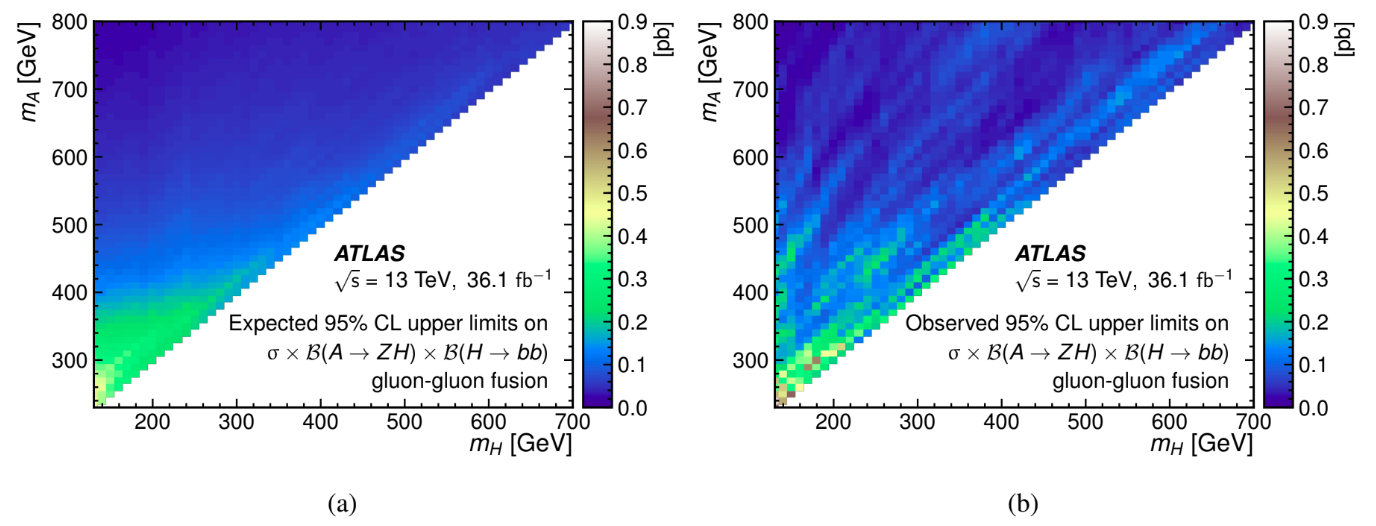
\includegraphics[width=1.0\textwidth]{Figs/confindence-levels.png}
    \end{figure}
    Upper bounds at 95\% CL on the production cross-section times the branching ratio $B(A\to ZH) \times B(H \to bb)$ in a pb for gluon-gluon fusion.
\end{frame}



\begin{frame}{Confidence Levels (2)}

\begin{figure}
    \centering
        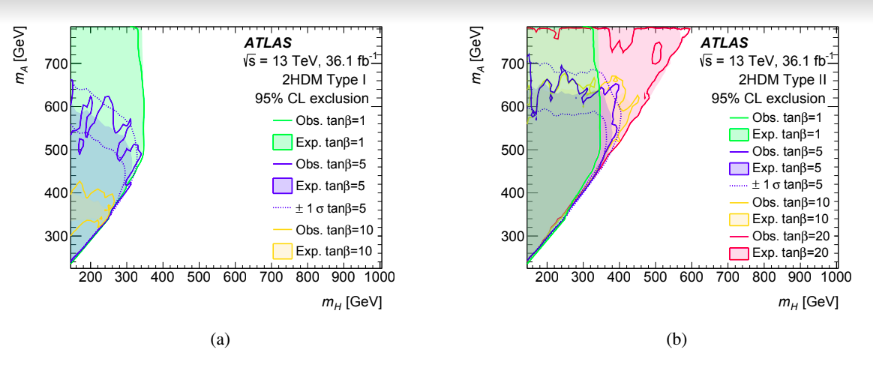
\includegraphics[width=1.0\textwidth]{Figs/available-regions-1.png}
    \end{figure}
        Observed and expected 95\% CL exclusion regions in the $(m_A, m_H)$ plane for various $\tan \beta$ values for (a) Type I, (b) Type II.

\end{frame}

\begin{frame}{Similar CMS search}

Four-body invariant mass distribution in the region of:
\begin{figure}%
    \centering
    \subfigure[low mass]{%
    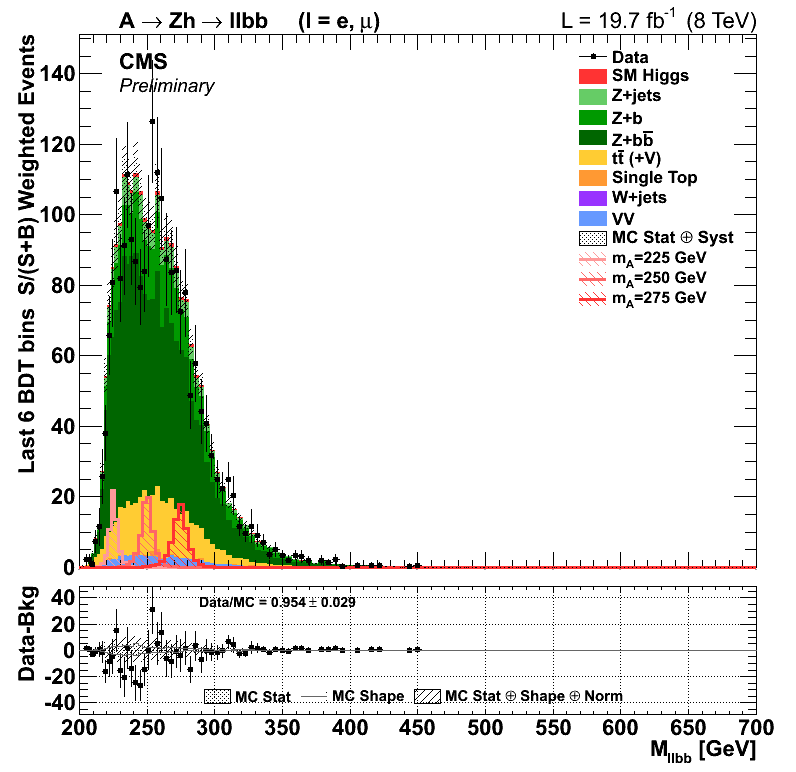
\includegraphics[height=1.25in]{Figs/cmssearch_low.png}}%
    \hfill
    \subfigure[intermediate mass]{%
    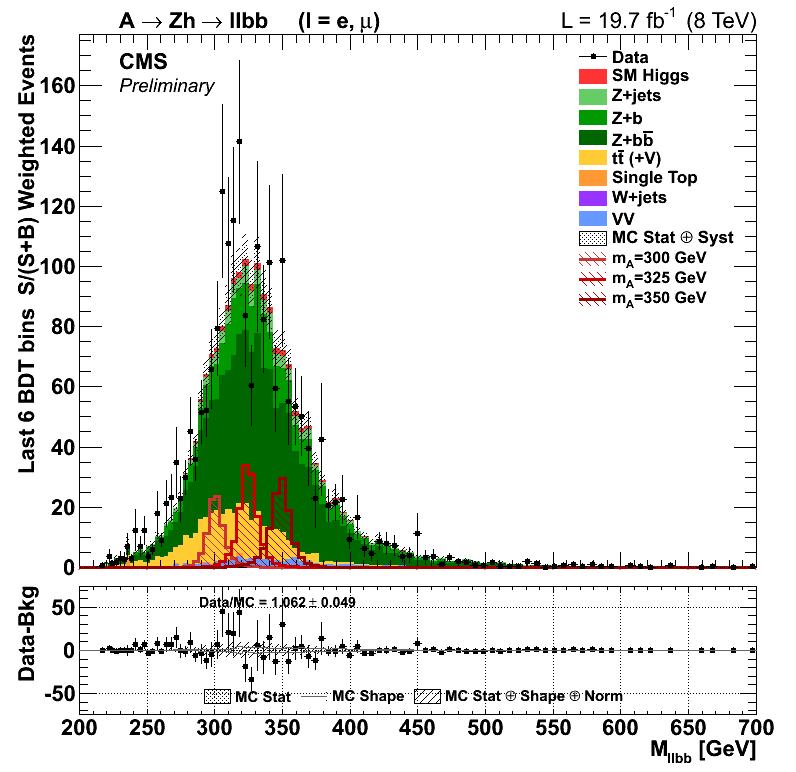
\includegraphics[height=1.25in]{Figs/cmssearch.png}}%
    \hfill
    \subfigure[high mass]{%
    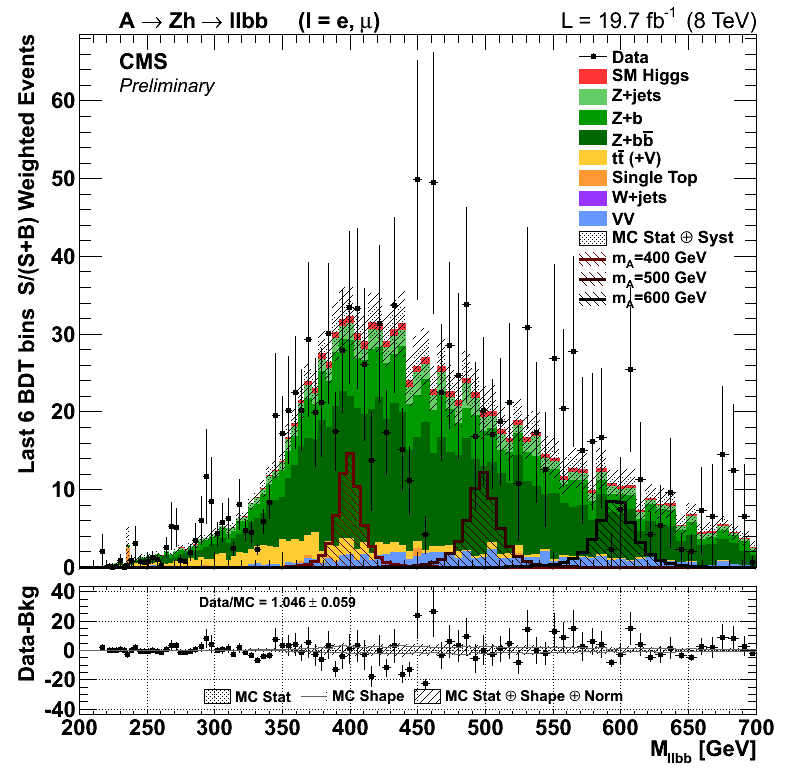
\includegraphics[height=1.25in]{Figs/cmssearch_high.png}}%
    \end{figure}
\begin{center}
    
\end{center}

\end{frame}


\begin{frame}{Summary}
    \begin{itemize}
        \uncover<1->{\item Search for a heavy Higgs boson, $A$, decaying into $ZH$, where $H$ denotes a heavy Higgs boson with mass $m_H > 125$ GeV.}
        \uncover<2->{\item A is assumed to be assumed to be produced via either gluon-gluon fusion or b-associated production}
        \uncover<3->{\item No significant deviation from the SM background predictions are observed in the $ZH \to \ell \ell b b$ final state}
        \uncover<4->{\item However, this search tightens the constraints on the 2HDM in the case of large mass splitting between its heavier neutral Higgs bosons}
    \end{itemize}

\end{frame}

\end{document}